%& /Users/ziky/.cache/org-persist/08/785fe3-55f8-449e-8551-e588336ca759-973d73c3c18746cbbc82919bce7e9bae
% Created 2025-09-12 Fri 17:35
% Intended LaTeX compiler: pdflatex
\documentclass[11pt]{article}
\usepackage[utf8]{inputenc}
\usepackage[T1]{fontenc}
\usepackage{amsmath}
\usepackage{amssymb}
\usepackage{capt-of}
\usepackage{hyperref}
\setlength{\abovedisplayskip}{0pt}
\setlength{\belowdisplayskip}{0pt}
\usepackage[a4paper, margin=1in]{geometry}

%% ox-latex features:
%   !announce-start, !guess-pollyglossia, !guess-babel, !guess-inputenc,
%   maths, image, !announce-end.

\usepackage{amsmath}
\usepackage{amssymb}

\usepackage{graphicx}

%% end ox-latex features


% end precompiled preamble
\ifcsname endofdump\endcsname\endofdump\fi

\author{Ziky Zhang}
\date{\today}
\title{MATH 110C notes}
\hypersetup{
 pdfauthor={Ziky Zhang},
 pdftitle={MATH 110C notes},
 pdfkeywords={},
 pdfsubject={},
 pdfcreator={},
 pdflang={English}}
\begin{document}

\maketitle
\tableofcontents

this note condensed \href{https://tutorial.math.lamar.edu/Classes/CalcIII/CalcIII.aspx}{Paul's Online Math Notes} that fits my need for understanding this class, so some details might be missing and some explanation might seems like random crap.

\newpage
\section{\href{https://tutorial.math.lamar.edu/Classes/CalcIII/3DSpace.aspx}{3-Dimensional Space}}
\label{sec:org8e4b995}
\subsection{\href{https://tutorial.math.lamar.edu/Classes/CalcIII/QuadricSurfaces.aspx}{Quadric Surfaces}}
\label{sec:orgef0c6e2}
\begin{itemize}
\item Ellipsoid
\end{itemize}
\[
\frac{x^2}{a^2} + \frac{y^2}{b^2} + \frac{z^2}{c^2} = 1
\]
Equation Explanation: \(x\), \(y\), \(z\) are all to the second degree, \(a\), \(b\), \(c\) are the distance from origin to \(x_{max}\), \(y_{max}\), \(z_{max}\), respectively.
\begin{center}
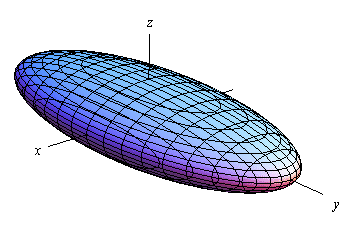
\includegraphics[width=6cm]{./img/1/ellipsoid.png}
\label{orgce6af6b}
\end{center}
;; NOTE: sphere is also a type of ellipsoid, that happens when \(a = b = c\).

\begin{itemize}
\item Cone
\end{itemize}
\begin{align*}
\frac{x^2}{a^2} + \frac{y^2}{b^2} &= \frac{z^2}{c^2} \\
\frac{x^2}{a^2} + \frac{y^2}{b^2} - \frac{z^2}{c^2} &= 0
\end{align*}
Equation Explanation: two of the three variables are positive and one is negative. the direction of the top and bottom are determined by negative variable, to both the positive and negative direction of that axis.
\begin{center}
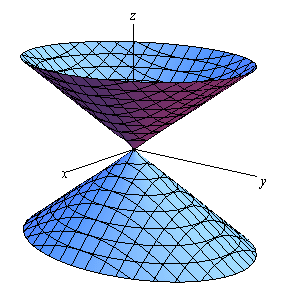
\includegraphics[width=6cm]{./img/1/cone.png}
\label{orgbbd5805}
\end{center}

\begin{itemize}
\item Cylinder
\end{itemize}
\begin{align*}
\frac{x^2}{a^2} + \frac{y^2}{b^2} = 1
\end{align*}
Equation Explanation: cylinders lacks one of the three variables, that means that the 2-D graph of the equation on their plane (xy-plane in this case) streches all the way on the missing axis (z-axis in this case).
\begin{center}
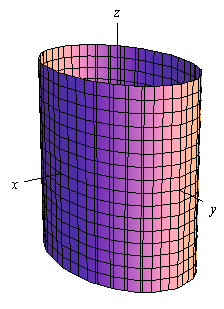
\includegraphics[width=6cm]{./img/1/cylinder.png}
\label{orge140baf}
\end{center}
;; NOTE: a cylinder doesn't have to be a enclosed 
\end{document}
